% This is LLNCS.DEM the demonstration file of
% the LaTeX macro package from Springer-Verlag
% for Lecture Notes in Computer Science,
% version 2.4 for LaTeX2e as of 16. April 2010
%
\documentclass{llncs}

% allows for temporary adjustment of side margins
\usepackage{chngpage}

% just makes the table prettier (see \toprule, \bottomrule, etc. commands below)
\usepackage{booktabs}

\usepackage[utf8]{inputenc}

% URL handling
\usepackage{url}
\urlstyle{same}

% footnotes
\usepackage{scrextend}

% Todos
%\usepackage[colorinlistoftodos]{todonotes}
%\newcommand{\ke}[1]{\todo[size=\small, color=orange!40]{\textbf{Kai:} #1}}
%\newcommand{\tb}[1]{\todo[size=\small, color=green!40]{\textbf{Thomas:} #1}}


%\usepackage{makeidx}  % allows for indexgeneration

%\usepackage{amsmath}
\usepackage{amsmath, amssymb}
\usepackage{mathabx}

% monospace within text
\newcommand{\ms}[1]{\texttt{#1}}

% examples
\usepackage{fancyvrb}
\DefineVerbatimEnvironment{ex}{Verbatim}{numbers=left,numbersep=2mm,frame=single,fontsize=\scriptsize}

\newenvironment{gcotable-1}{
  \scriptsize
  \sffamily
  \vspace{0.3cm}
  \begin{tabular}{l|l|l|l|l|l}
  \hline
  \textbf{c. type} & \textbf{context concept} & \textbf{p. list} & \textbf{concepts} & \textbf{c. element} & \textbf{c. value} \\
  \hline

}{
  \hline
  \end{tabular}
  \linebreak
}

\newenvironment{gcotable}{
  \scriptsize
  \sffamily
  \vspace{0.3cm}
	\begin{center}
  \begin{tabular}{l|l|l|l|l|l|l}
  \hline
  \textbf{c. type} & \textbf{context class} & \textbf{left p. list} & \textbf{right p. list} & \textbf{classes} & \textbf{c. element} & \textbf{c. value} \\
  \hline

}{
  \hline
  \end{tabular}
	\end{center}
}

\newenvironment{DL}{
  %\scriptsize
  %\sffamily
  %\vspace{0.3cm}
	\begin{center}
  \begin{tabular}{r l}

}{
  \end{tabular}
	\end{center}
}

\newenvironment{evaluation}{
  %\scriptsize
  %\sffamily
  %\vspace{0.3cm}
	\begin{center}
  \begin{tabular}{l|c|c|c|c|c|c}
  \hline
  \textbf{Constraint Class} & \textbf{DSP} & \textbf{OWL2-DL} & \textbf{OWL2-QL} & \textbf{ReSh} & \textbf{ShEx} & \textbf{SPIN} \\
  \hline

}{
  \hline
  \end{tabular}
	\end{center}
}

\newenvironment{evaluation-generic-overview}{
  %\scriptsize
  %\sffamily
  %\vspace{0.3cm}
	\begin{center}
  \begin{tabular}{l|c|c}
  \hline
  \textbf{Constraint Classes} & \textbf{\#} & \textbf{\%} \\
  \hline

}{
  \hline
  \end{tabular}
  \linebreak
	\end{center}
}

\usepackage{xspace}
% Einfache und doppelte Anfuehrungszeichen
\newcommand{\qs}{``} 
\newcommand{\qe}{''\xspace} 
\newcommand{\sqs}{`} 
\newcommand{\sqe}{'\xspace} 

% checkmark
\usepackage{tikz}
\def\checkmark{\tikz\fill[scale=0.4](0,.35) -- (.25,0) -- (1,.7) -- (.25,.15) -- cycle;} 

% Xs
\usepackage{pifont}

% Tabellenabstände kleiner
\setlength{\intextsep}{10pt} % Vertical space above & below [h] floats
\setlength{\textfloatsep}{10pt} % Vertical space below (above) [t] ([b]) floats
% \setlength{\abovecaptionskip}{0pt}
% \setlength{\belowcaptionskip}{0pt}

\usepackage{tabularx}
\newcommand{\hr}{\hline\noalign{\smallskip}} % für die horizontalen linien in tabellen

% pipe
%\usepackage[T1]{fontenc}

% Todos
\usepackage[colorinlistoftodos]{todonotes}
\newcommand{\ke}[1]{\todo[size=\small, color=orange!40]{\textbf{Kai:} #1}}
\newcommand{\tb}[1]{\todo[size=\small, color=green!40]{\textbf{Thomas:} #1}}

\setcounter{secnumdepth}{5}

\begin{document}

%
%
\title{Formulating and Validating RDF Constraints Generically}
%\subtitle{}
%
\titlerunning{XXXXX}  % abbreviated title (for running head)
%                                     also used for the TOC unless
%                                     \toctitle is used
%
\author{Thomas Bosch\inst{1} \and X\inst{2} \and X\inst{2} \and X\inst{2} \and Kai Eckert\inst{2}}
%
\authorrunning{XXXXX} % abbreviated author list (for running head)
%
%%%% list of authors for the TOC (use if author list has to be modified)
\institute{GESIS – Leibniz Institute for the Social Sciences, Germany\\
\email{thomas.bosch@gesis.org},\\ 
\and
University of Mannheim, Germany \\
\email{\{kai\}@informatik.uni-mannheim.de} 
}

\maketitle              % typeset the title of the contribution

\begin{abstract}


\keywords{..}
\end{abstract}
%

% ---------------

\section{Introduction}

\begin{itemize}
	\item requirements database
	\item relationship between requirements and constraints
	\item constraint languages
\end{itemize}

\section{Ideas}

\begin{itemize}
	\item the majority of specific constraints expressed by any specific constraint language can be expressed by DL
	\item each DL statement can be expressed by a generic constraint using a generic constraint language
\end{itemize}

purpose:
\begin{itemize}
	\item translations of specific constraints expressed by any specific constraint language
	\item we do not invent a new constraint languages
\end{itemize}

%constraint design patterns:
% - ontology design pattern.org
% - DSP uses other design pattern
% - constraint elements are the same / 
% - constraint / constraint elements / constraint design patterns / constraint language

%dependency between requirements / when this requirements is fulfilled then this is also fulfilled (e.g. min card and requ. car)
%min car more powerful than req. propery

\begin{itemize}
	\item any specific constraint (expressed by specific constraint language) must be mapped to a generic constraint (expressed by GCL)
\end{itemize}

\section{Motivation}

Cardinality restrictions can be expressed either generically by description logics (DL) (\ms{generic constraints}) and additional constraints or specifically (\ms{specific constraints}) by domain-specific constraint languages such as OWL 2, DSP, ShEx, ReSh, and SPIN.
With minimum qualified cardinality restrictions we can state, e.g., that a star fleet captain commands at least one vessel, which may be represented by DL in a logical way:

\begin{DL}
$StarFleetCaptain \sqsubseteq \geq1 commandsVessel . Vessel $
\end{DL}

The same constraint may also be represented by different constraint languages like OWL 2, ShEx, ReSh, or DSP:

\begin{ex}
# OWL 2
# -----
StarFleetCaptain
    a owl:Restriction ;
    owl:minQualifiedCardinality 1 ;
    owl:onProperty commandsVessel ;
    owl:onClass Vessel .
		
# ShEx
# ----
StarFleetCaptain { commandsVessel @Vessel{1, } }

# ReSh
# ----
StarFleetCaptain a rs:ResourceShape ; rs:property [
    rs:name "commandsVessel" ; rs:propertyDefinition commandsVessel ;
    rs:valueShape Vessel ;
    rs:occurs rs:One-or-many ; ] .
				
# DSP
# ---			
descriptionTemplate a dsp:DescriptionTemplate ; 
    dsp:resourceClass StarFleetCaptain ; 
    dsp:statementTemplate [ a dsp:NonLiteralStatementTemplate ;
        dsp:minOccur 1 ; dsp:maxOccur "infinity" ; 
        dsp:property commandsVessel ; 
        dsp:nonLiteralConstraint [ a dsp:NonLiteralConstraint ;
            dsp:valueClass Vessel ] ] .
\end{ex}

As \ms{Janeway} commands the vessel \ms{Voyager} (\ms{commandsVessel(Janeway,Voyager)}) and \ms{Voyager} is defined to be a \ms{Vessel} (\ms{rdf:type(Voyager,Vessel)}), the assignment of \ms{Janeway} to the class \ms{StarFleetCaptain} (\ms{rdf:type(Janeway,StarFleetCaptain)}) does not cause any constraint violation.
A constraint violation is raised, however, when there is no \ms{commandsVessel} relationship pointing from the individual \ms{Janeway}. 
A constraint violation is also raised, when there is a triple \ms{commandsVessel(Janeway,Voyager)}, but \ms{Voyager} is not explicitly defined to be a \ms{Vessel}, 
i.e. the triple \ms{rdf:type(Voyager,Vessel)} is not present in the data. 
As the object of the \ms{commandsVessel} property is assigned to another class than \ms{Vessel}, 
the triples \ms{commandsVessel(Sisko,DS9)}, \ms{rdf:type(Sisko,StarFleetCaptain)}, and \ms{rdf:type(DS9,SpaceStation)}  
also cause a constraint violation.

As there is no standard constraint language, constraint designers may choose different constraint languages to express the identical cardinality restriction. 
When constraint designers choose one constraint language to express an arbitrary constraint, it should be possible to transform this constraint into a constraint expressed by any other constraint language. 
This is important as it is often the case that one constraint designer knows to read and to write constraints in one constraint language very well but not in another constraint language. 
This way, constraint designers may communicate with each other without the necessity to understand all constraint languages and the interoperability of constraint languages is enhanced.


There are validation environments available enabling to automatically validate RDF constraints expressed by just a few constraint languages such as OWL 2\footnote{\url{purl.org/net/rdfval-demo}\label{footnote1}}, DSP\footref{footnote1}, and ShEx\footnote{\url{http://www.w3.org/2013/ShEx/FancyShExDemo}}.
It should be possible to validate any RDF constraints expressed by any constraint language automatically and what is even more important in exactly the same manner without any differences.  

The following table shows the mapping between the cardinality restriction expressed in DL and the cardinality restriction (\ms{generic constraint}) expressed by a generic constraint language conforming to an ontology to describe any RDF constraint generically (see section~\ref{sec:ontology}).
Each constraint is either a constraint on classes or a constraint on properties.

\begin{gcotable}
property & Captain & commandsVessel & - & Vessel & $\geq$ & 1 \\
\end{gcotable}

The cardinality restriction (expressed by the generic constraint language) is represented in RDF as follows:

\begin{ex}
[   a PropertyConstraint ;
    contextClass StarFleetCaptain ;
    leftProperties ( commandsVessel ) ;
    classes ( Vessel ) ;
    constrainingElement ">=" ;
    constrainingValue "1" ] .
\end{ex}

We implemented the automatic validation for the cardinality restriction expressed by the generic constraint language within our SPIN validation environment (see SPARQL query above):

\begin{ex}
# constraint
# ----------
[   a PropertyConstraint ;
    contextClass ?cc ;
    leftProperties ( ?p1 ) ;
    classes ( ?c1 ) ;
    constrainingElement ">=" ;
    constrainingValue ?cv ] .
		
# data
# ----
?subject rdf:type ?cc .

# validation
# -----
BIND ( qualifiedCardinality( ?subject, ?p1, ?c1 ) AS ?c ) .
FILTER ( ?c < ?cv ) .		  
\end{ex}

If we transform a specific constraint (expressed by any constraint language) into a generic constraint (expressed by the generic constraint language), we will be able to validate the generic constraint and therefore the specific constraint immediately. 
As a consequence, we do not have to specify an automatic validation for each specific constraint, as we need to define an automatic validation only once for each generic constraint. 
We have to provide an automatic validation for each generic constraint in order to support the automatic validation for each specific constraint.

When domain experts use graphical user interfaces to define constraints in a user-friendly way (without the necessity to express constraints on their own), 
constraints can be mapped to either a specific or a generic constraint, as for both an automatic validation is provided in the background.    
So, the user does not have to know how to express specific constraints using any constraint language.
If there is a new constraint not covered by any existing constraint language, one can just define the automatic validation for a corresponding generic constraint.
This way, one is able to extend existing constraint languages and also to define new constraint languages if existing constraint languages are not sufficient to express particular constraints.
If a language designer develops a new constraint language, 
the language designer only needs to define a mapping between the new constraint language and the generic constraint language
in order to be able to automatically validate the constraints expressible by the new constraint language.

The \textbf{contributions} of this paper are:
\begin{itemize}
	%\item Any specific constraint (expressed by any constraint language) can be transformed into a generic constraint (expressed by the generic constraint language)
	%\item Any specific constraint (expressed by any constraint language A) can be transformed into any specific constraint (expressed by any constraint language B)
	%\item Any specific constraint (expressed by any constraint language) can be validated automatically (if an automatic validation is defined only once for corresponding generic constraint)
	\item We define a terminology for RDF constraints and constraining languages
	\item We developed an ontology describing any RDF constraint which can also be expressed by any constraint language
	\item We present that any RDF constraint can be described by the developed ontology - whether the constraint can be expressed in DL or not 
	\item We show how to transform specific constraints (expressed by any constraint language A) into generic constraints and into specific constraints (expressed by any other constraint language B)
  \item We explain that any specific constraint can be validated automatically (if an automatic validation is defined only once for corresponding generic constraint)
\end{itemize}

%The \textbf{benefits} of our framework are:
%\begin{itemize}
	%\item Any specific constraint (expressed by any constraint language) can be transformed into a generic constraint (expressed by the generic constraint language)
	%\item Any specific constraint (expressed by any constraint language A) can be transformed into any specific constraint (expressed by any constraint language B)
	%\item Any specific constraint (expressed by any constraint language) can be validated automatically (if an automatic validation is defined only once for corresponding generic constraint)
%\end{itemize}

\textcolor{red}{paper organization}

\section{An Ontology Describing RDF Constraints Generically} 
\label{sec:ontology}

We developed a very simple ontology (three classes, three object properties, and three data properties) which is universal enough to describe any RDF constraint expressible by any RDF constraint language.
We distinguish between two sub-types of \ms{constraint}: 
\begin{itemize}
	\item \ms{property constraints} and 
	\item \ms{class constraints}. 
\end{itemize}

For both property and class constraints a context class, a list of classes, the constraining element, and the constraining value can be stated
(see figure \ref{fig:generic-constraint-language-ontology}). Lists of left and right properties can only be stated for property constraints.

\begin{figure}
	\centering
		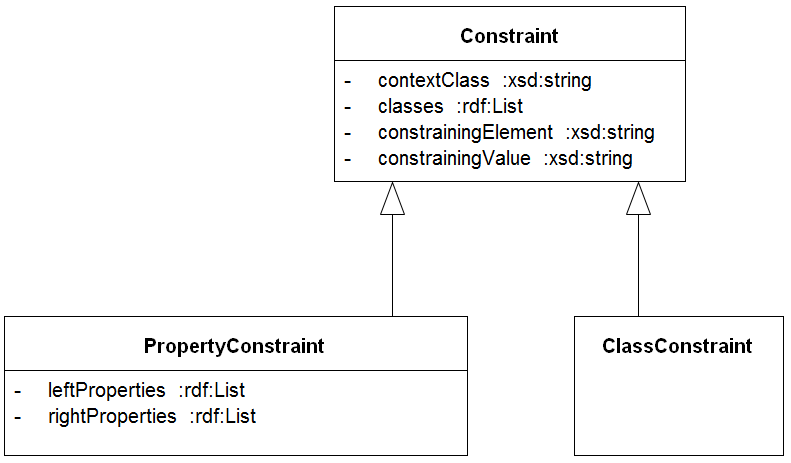
\includegraphics[width=0.80\textwidth]{images/generic-constraint-language-ontology.png}
	\caption{generic constraint language ontology}
	\label{fig:generic-constraint-language-ontology}
\end{figure}

In order to define this ontology, it is needed to define the terminology for the formulation of constraints. 
A \ms{constraint language} is a language which is used to formulate constraints.
The W3C Data Shapes WG defines \ms{constraint} as a component of a schema what needs to be satisfied\footnote{\url{https://www.w3.org/2014/data-shapes/wiki/Glossary}}.
A constraint holds for all individuals of a context class (\ms{contextClass}).
Consider, e.g., the following cardinality restriction on the property \ms{commandsVessel}, which restricts that a captain must command at least one vessel: 
\begin{DL}
$Captain \sqsubseteq \geq1 commandsVessel . Vessel $
\end{DL}
Mapped to the GCLO the cardinality restriction is classified as a property constraint which holds for individuals of the class \ms{Captain} - the context class:
\begin{gcotable}
property & Captain & commandsVessel & - & Vessel & $\geq$ & 1 \\
\end{gcotable}
The constraining element (\ms{constrainingElement}) is the operator indicating the actual type of constraint like DL concept and role constructors, (in)equality, and further keywords for constrains which cannot be expressed in DL (e.g. regular expressions, constraining facets).
In some cases, a constraint is only complete when in addition to the constraining element a constraining value (\ms{constrainingValue}) is stated.
The cardinality restriction 
\begin{DL}
$\geq$1 commandsVessel . Vessel
\end{DL}
constructs an anonymous class of all individuals who command at least one vessel.
Thus, the constraining element of this property constraint is the DL at-least restriction \ms{$\geq$} and the constraining value is \ms{1}.
\ms{Classes} indicate the list of classes constraints refer to.
In case of the property constraint above, the qualified cardinality restriction refers to the class \ms{Vessel}, 
i.e., restricting the objects, the property \ms{commandsVessel} point to, to be of the class \ms{Vessel}.

\section{Complex Constraints}

\ms{Complex constraints} encompass complex constraints and/or \ms{simple constraints} (atomic constraints).
DL statements of complex constraints are created out of DL statements of composed constraints. 

\textbf{Context-Specific Exclusive OR of Property Groups}\footnote{corresponds to R-13-DISJOINT-GROUP-OF-PROPERTIES-CLASS-SPECIFIC}\textbf{.}
Exclusive or is a logical operation that outputs true whenever both inputs differ (one is true, the other is false).
Only one of multiple property groups should be present in the data.
Half-Klingons, e.g., either have a klingon mother and a human father or a human mother and a klingon father, which can be expressed by ShEx:

\begin{ex}
Half-Klingon { 
    ( klingonMother Klingon , humanFather Human ) |
    ( humanMother Human , klingonFather Klingon ) }
\end{ex}

As \ms{B'Elanna Torres} is a \ms{Half-Klingon} with a klingon mother and a human father, this data is valid:

\begin{ex}
BElannaTorres a Half-Klingon ;
    klingonMother Miral ; humanFather JohnTorres .
\end{ex}

%\begin{DL}
%rdf:type(BElannaTorres,Half-Klingon) \\
%klingonMother(BElannaTorres,Miral) \\
%klingonMother(BElannaTorres,JohnTorres)
%\end{DL}

This complex constraint can be mapped to DL:

\begin{DL}
Half-Klingon $\sqsubseteq$ ($\neg$E $\sqcap$ F) $\sqcup$ (E $\sqcap$ $\neg$F) \\ 
E $\equiv$ A $\sqcap$ B \\
F $\equiv$ C $\sqcap$ D \\
A $\sqsubseteq$ $\geq$ 1 klingonMother.Klingon $\sqcap$ $\leq$ 1 klingonMother.Klingon \\
B $\sqsubseteq$ $\geq$ 1 humanFather.Human $\sqcap$ $\leq$ 1 humanFather.Human \\
C $\sqsubseteq$ $\geq$ 1 humanMother.Human $\sqcap$ $\leq$ 1 humanMother.Human \\
D $\sqsubseteq$ $\geq$ 1 klingonFather.Klingon $\sqcap$ $\leq$ 1 klingonFather.Klingon \\
\end{DL}

The constraint expressed by DL can be mapped to a generic constraint:

\begin{gcotable}
class & Half-Klingon & - & - & $\neg$E $\sqcap$ F, E $\sqcap$ $\neg$F & $\sqcup$ & - \\
class & $\neg$E $\sqcap$ F & - & - & $\neg$E, F & $\sqcap$ & - \\
class & E $\sqcap$ $\neg$F & - & - & E, $\neg$F & $\sqcap$ & - \\
class & $\neg$E & - & - & E & $\neg$ & - \\
class & E & - & - & A, B & $\sqcap$ & - \\
class & $\neg$F & - & - & F & $\neg$ & - \\
class & F & - & - & C, D & $\sqcap$ & - \\
class & A & - & - & A1, A2 & $\sqcap$ & - \\
property & A1 & klingonMother & - & Klingon & $\geq$ & 1 \\
property & A2 & klingonMother & - & Klingon & $\leq$ & 1 \\
class & B & - & - & B1, B2 & $\sqcap$ & - \\
property & B1 & humanFather & - & Human & $\geq$ & 1 \\
property & B2 & humanFather & - & Human & $\leq$ & 1 \\
class & C & - & - & C1, C2 & $\sqcap$ & - \\
property & C1 & humanMother & - & Human & $\geq$ & 1 \\
property & C2 & humanMother & - & Human & $\leq$ & 1 \\
class & D & - & - & D1, D2 & $\sqcap$ & - \\
property & D1 & klingonFather & - & Klingon & $\geq$ & 1 \\
property & D2 & klingonFather & - & Klingon & $\leq$ & 1 \\
\end{gcotable}

Even though, tools may generate generic constraints automatically, this complex constraint is composed of many other complex (e.g. minimum and maximum qualified cardinality restrictions) and simple constraints (e.g. constraints on sets).
As \ms{exact (un)qualified cardinality restrictions} and \ms{exclusive or} are frequently used complex constraints,
we propose using them as simple constraints - 	in terms of syntactic sugar.
As a consequence, the \ms{Context-Specific Exclusive OR of Property Groups} constraint above is represented as a generic constraint more intuitively and concisely:

\begin{gcotable}
class & Half-Klingon & - & - & E, F & XOR \\
class & E & - & - & A, B & $\sqcap$ \\
class & F & - & - & C, D & $\sqcap$ \\
property & A & klingonMother & - & Klingon & = & 1 \\
property & B & humanFather & - & Human & = & 1 \\
property & C & humanMother & - & Human & = & 1 \\
property & D & klingonFather & - & Klingon & = & 1 \\
\end{gcotable}

\subsection{Disjoint Classes}

\begin{DL}
Hologram $\sqcap$ Human $\sqsubseteq$ $\perp$\\
Alternative:\\
$Hologram \sqsubseteq \neg Human$
\end{DL}

\subsection{Minimum Qualified Cardinality Restrictions on Properties}

\begin{DL}
$FederationCaptain \sqsubseteq Federation \sqcap \geq1 commandsVessel . Vessel $
\end{DL}

\section{Syntactic Sugar}

\begin{itemize}
	\item syntactic sugar for some constraints
\end{itemize}

In Section 1.3 we introduced three forms of RBox axioms: role inclusions, role equiv-
alences and role disjointness. OWL provides a variety of others, namely role transi-
tivity, symmetry, asymmetry, reflexivity and irreflexivity. These are sometimes consid-
ered as basic axiom types in DLs as well, using some suggestive notation such as
Trans( ancestorOf ) to express that the role ancestorOf is transitive. However, such axioms
are just syntactic sugar; all role characteristics can be expressed using the features
of DLs that we have already introduced.

\begin{itemize}
  \item domain and range
	\item Primary Key Properties
	\item (ir)reflexive object properties
	\item ( Exact Qualified Cardinality Restrictions on Properties )
\end{itemize}

\section{Transformations between Specific Constraints}

\section{Automatic Validation of Specific Constraints}

\section{Simple Constraints Not Expressible in DL}

There are simple constraints which cannot be expressed by DL such as literal pattern matching, literal value comparison, literal ranges, default values, and language tag cardinality \cite{BoschNolleAcarEckert2015}.

% maybe additional constraint default values:
% ear shape of races, e.g. vulcans / teeth color
% mathematical operations

There are multiple use cases associated with the requirement to match literals according to given patterns (\ms{Literal Pattern Matching} constraint).
The enterprise vessel, e.g.,  can only have the registry numbers "NCC-1701", "NCC-1701-A", "NCC-1701-B", "NCC-1701-C", "NCC-1701-D", or "NCC-1701-E".
The universal restriction part of this complex constraint can be expressed by OWL 2 DL:
\ms{Enterprise $\sqsubseteq$ $\forall$ registryNumber.RegistryNumber}.
The restriction of the datatype \ms{RegistryNumber}, however, cannot be expressed in DL, but OWL 2 DL can be used anyway to express the literal pattern matching constraint:

\begin{ex}
RegistryNumber
    a rdfs:Datatype ;
    owl:equivalentClass [
        a rdfs:Datatype ;
        owl:onDatatype xsd:string ;
        owl:withRestrictions ( 
            [ xsd:pattern "NCC-1701([-][A-E])?" ] ) ] .
\end{ex}

The second axiom defines \ms{RegistryNumber} as an abbreviation for a datatype restriction on \ms{xsd:string}. 
The first axiom explicitly declares \ms{RegistryNumber} to be a datatype. 
The datatype \ms{RegistryNumber} can be used just like any other datatype like in the universal restriction above.
The literal pattern matching constraint validates \ms{RegistryNumber} literals according to the stated regular expression causing a constraint violation for the triples 
\ms{Janeway commandsEnterprise Voyager} and \ms{Voyager registryNumber "NCC-74656"\textasciicircum{}\textasciicircum{}RegistryNumber}, 
but not for the triples \ms{Picard commandsEnterprise Enterprise} and \ms{Enterprise registryNumber "NCC-1701-E"\textasciicircum{}\textasciicircum{}RegistryNumber}.
The universal restriction and the literal pattern matching constraint are mapped to the generic constraint language as follows:

\begin{gcotable}
property & Enterprise & registryNumber & - & RegistryNumber & $\forall$ & - \\
class & RegistryNumber & - & - & xsd:string & regex & 'NCC-1701([-][A-E])?' \\
\end{gcotable}

The \ms{Literal Pattern Matching} constraint introduces a new constraining element: \ms{regex}.
For this new constraining element, an automatic validation must be implemented in SPIN.
This has to be done once for each constraint which cannot be expressed in DL.

\section{Implementation}

SPARQL is generally seen as the method of choice to validate RDF data according to certain constraints, although it is not ideal for their formulation. 
In contrast, OWL 2 and DSP constraints are comparatively easy to understand, but lack an implementation to validate RDF data. 
Bosch and Eckert\cite{BoschEckert2014-2} use SPIN as basis to define a
validation environment in which the validation of any constraint language\footnote{the only limitation is that constraint languages must be represented in RDF} can be implemented by representing them in SPARQL. 
The validation implementation of constraint languages is fully declarative,
consisting of a mapping from constraint languages to SPIN in form of SPARQL CONSTRUCT queries.
SPIN represents both the SPIN mappings and the SPARQL queries in RDF. 
Within the validation environment, we fully implemented an automatic validation of all OWL 2 DL\footnote{OWL 2 SPIN mapping: \url{https://github.com/boschthomas/OWL2-SPIN-Mapping}} and DSP\footnote{DSP SPIN mapping: \url{https://github.com/dcmi/DSP-SPIN-Mapping}} constructs (for the complete DSP validation see \cite{BoschEckert2014-2}). 
The implementation can be tested at \url{http://purl.org/net/rdfval-demo}.
The SPIN engine checks for each resource if it satisfies all constraints (associated with its assigned classes) and generates a result RDF graph containing information about all constraint violations.

We provide a mapping from the generic constraint language to SPIN\footnote{GCL SPIN mapping: \url{https://github.com/boschthomas/GCL-SPIN-Mapping}} in order to automatically validate each type of generic constraint (simple, complex, property, and class constraints).
Part of future work will be 
\begin{itemize}
	\item to provide a GUI which generates generic constraints automatically according to inputs of domain experts who are not familiar with the formulation of constraints.
	\item to extend our RDF validator to provide bidirectional transformations between specific constraints (expressed by multiple constraint languages) and generic constraints. 
\end{itemize}

\section{Evaluation}

We evaluated to which extend the most promising five constraint languages fulfill each of the overall 74 requirements to formulate RDF constraints \cite{BoschNolleAcarEckert2015}.
If a constraint can be expressed in DL, we added the mapping to DL and to the generic constraint.
If a constraint cannot be expressed in DL, we added a mapping to the generic constraint.
Therefore, we show that each constraint can be mapped to a generic constraint.
The following table shows the absolute number and the relative percentage for the three dimensions to classify constraints:

\begin{evaluation-generic-overview}
Property Constraints & 48 & 65 (64.86) \\
Class Constraints & 17 & 23 (22.96) \\
Property and Class Constraints & 9 & 12 (12.16) \\
\hline
Simple Constraints & 46 & 62 (62.16) \\
Simple Constraints (Syntactic Sugar) & 10 & 14 (13.51) \\
Complex Constraints & 18 & 24 (24.32) \\
\hline
DL Expressible & 51 & 69 (68.92) \\
DL Not Expressible & 23 & 31 (31.08) \\
\hline
Total & 74 & 100 \\
\end{evaluation-generic-overview}

Constraints can be classified as \ms{property constraints} and \ms{class constraints}.
Two thirds are property constraints, one fifth class constraints, and approx. 10\% are composed of both property and class constraints.
Constraints may be either atomic (\ms{simple constraints}) or created out of simple and complex constraints (\ms{complex constraints}).
Almost two thirds are simple constraints, a quarter are complex constraints.
Almost 15 percent are complex constraints which can be formulated as simple constraints when used in terms of syntactic sugar.
Constraints can either be expressible in DL or not.
Nearly 70\% of the overall constraints are expressible in DL.	

\section{Related Work}

\section{Conclusion and Future Work}

\bibliography{../../literature/literature}{}
\bibliographystyle{plain}
\setcounter{tocdepth}{1}
%\listoftodos
\end{document}
